\subsection{Análise de Requisitos}


\subsubsection{Requisito 1 - Cadastro de Novos Clientes:} O sistema deve permitir que novos clientes se cadastrem fornecendo informações pessoais, como nome e endereço de e-mail. Essa funcionalidade é essencial para identificar e distinguir os usuários do sistema.

\subsubsection{Requisito 2 - Selecionar Cidades ou Atrações do Roteiro:} Os clientes devem poder selecionar as cidades ou atrações turísticas que desejam incluir em seus roteiros de viagem. Essa funcionalidade visa permitir que os clientes personalizem seus roteiros com base em seus interesses específicos.

\subsubsection{Requisito 3 - Acessar a API do Google para Coletar Dados sobre as Cidades:} O sistema precisa acessar a API do Google para obter informações atualizadas e relevantes sobre as cidades e atrações turísticas selecionadas pelos clientes. Esses dados são fundamentais para a otimização das rotas.

\subsubsection{Requisito 4 - Formatar e Computar os Dados Adquiridos:} Os dados coletados da API do Google devem ser formatados e computados adequadamente para permitir a otimização das rotas. Essa funcionalidade é responsável por preparar os dados para o Sistema de Otimização.

\subsubsection{Requisito 5 - Otimizar Rotas:} O sistema deve otimizar as rotas turísticas com base nas preferências dos clientes e nas informações das cidades ou atrações. Essa funcionalidade visa criar itinerários eficientes que maximizem a satisfação dos clientes.

\subsubsection{Requisito 6 - Elaborar Relatórios sobre Rotas:} O Sistema de Otimização deve ser capaz de elaborar relatórios detalhados sobre as rotas turísticas otimizadas. Esses relatórios fornecem informações valiosas sobre os itinerários gerados, permitindo análises e tomadas de decisões mais informadas.

\subsubsection{Requisito 7 - Consultar Relatórios sobre as Rotas:} Os clientes e o Administrador do Sistema devem poder consultar os relatórios sobre as rotas turísticas otimizadas. Essa funcionalidade permite que os usuários tenham acesso às informações relevantes e auxilia na avaliação da eficiência do sistema.

\subsubsection{Requisito 8 - Armazenar Rotas Já Otimizadas em uma Base de Dados:} O Sistema de Coleta de Dados deve ser capaz de armazenar as rotas turísticas já otimizadas em uma base de dados. Essa funcionalidade é importante para garantir que os itinerários anteriores sejam mantidos para futuras consultas e referências.

\subsubsection{Requisito 9 - Disponibilizar Informações sobre as Cidades:} A API do Google deve disponibilizar informações detalhadas sobre as cidades e atrações turísticas para que os clientes possam fazer suas seleções de forma adequada. Essa funcionalidade é fundamental para fornecer dados precisos e atualizados para o processo de otimização.

\subsubsection{Requisito 10 - Enviar Feedbacks:} Os clientes devem poder enviar feedbacks sobre os roteiros turísticos e a experiência geral com o sistema. Essa funcionalidade permite que os usuários expressem suas opiniões e sugestões para aprimoramento contínuo do sistema.

\subsubsection{Requisito 11 - Armazenar Dados do Cliente e dos Feedbacks:} O Sistema de Feedback deve ser capaz de armazenar os dados dos clientes cadastrados e os feedbacks enviados por eles. Essa funcionalidade é importante para garantir a persistência dos dados e possibilitar análises futuras.

\subsubsection{Requisito 12 - Elaborar Relatório sobre Feedbacks:} O Sistema de Feedback deve elaborar relatórios detalhados sobre os feedbacks enviados pelos clientes. Esses relatórios são valiosos para a análise das sugestões e experiências relatadas pelos usuários.

\subsection{Diagrama de Caso de Uso}

O diagrama de caso de uso é uma ferramenta essencial na engenharia de requisitos, permitindo uma representação visual das interações entre os atores externos e as funcionalidades oferecidas pelo sistema. Nesta seção, apresentaremos o diagrama de caso de uso que descreve as principais funcionalidades do sistema de otimização de roteiros turísticos.

O diagrama de caso de uso identifica os atores envolvidos no sistema, representados por \textit{clientes} e \textit{administrador do sistema}, e detalha as interações entre eles e o sistema. Além disso, apresenta as funcionalidades oferecidas, como o cadastro de novos clientes, a seleção de cidades ou atrações turísticas, a otimização de rotas, a consulta de relatórios sobre as rotas e a possibilidade de enviar feedbacks.

Essa representação visual do sistema de otimização de roteiros turísticos é crucial para compreender claramente suas funcionalidades e requisitos, bem como para identificar os fluxos de interação entre os atores e o sistema. Na figura, \ref{fig:DCU} há uma miniatura do diagrama, que pode ser melhor consultado no apêdice.


\begin{figure}[H]
    \centering
    \caption{Diagrama de Caso de Uso}
    \label{fig:DCU}
    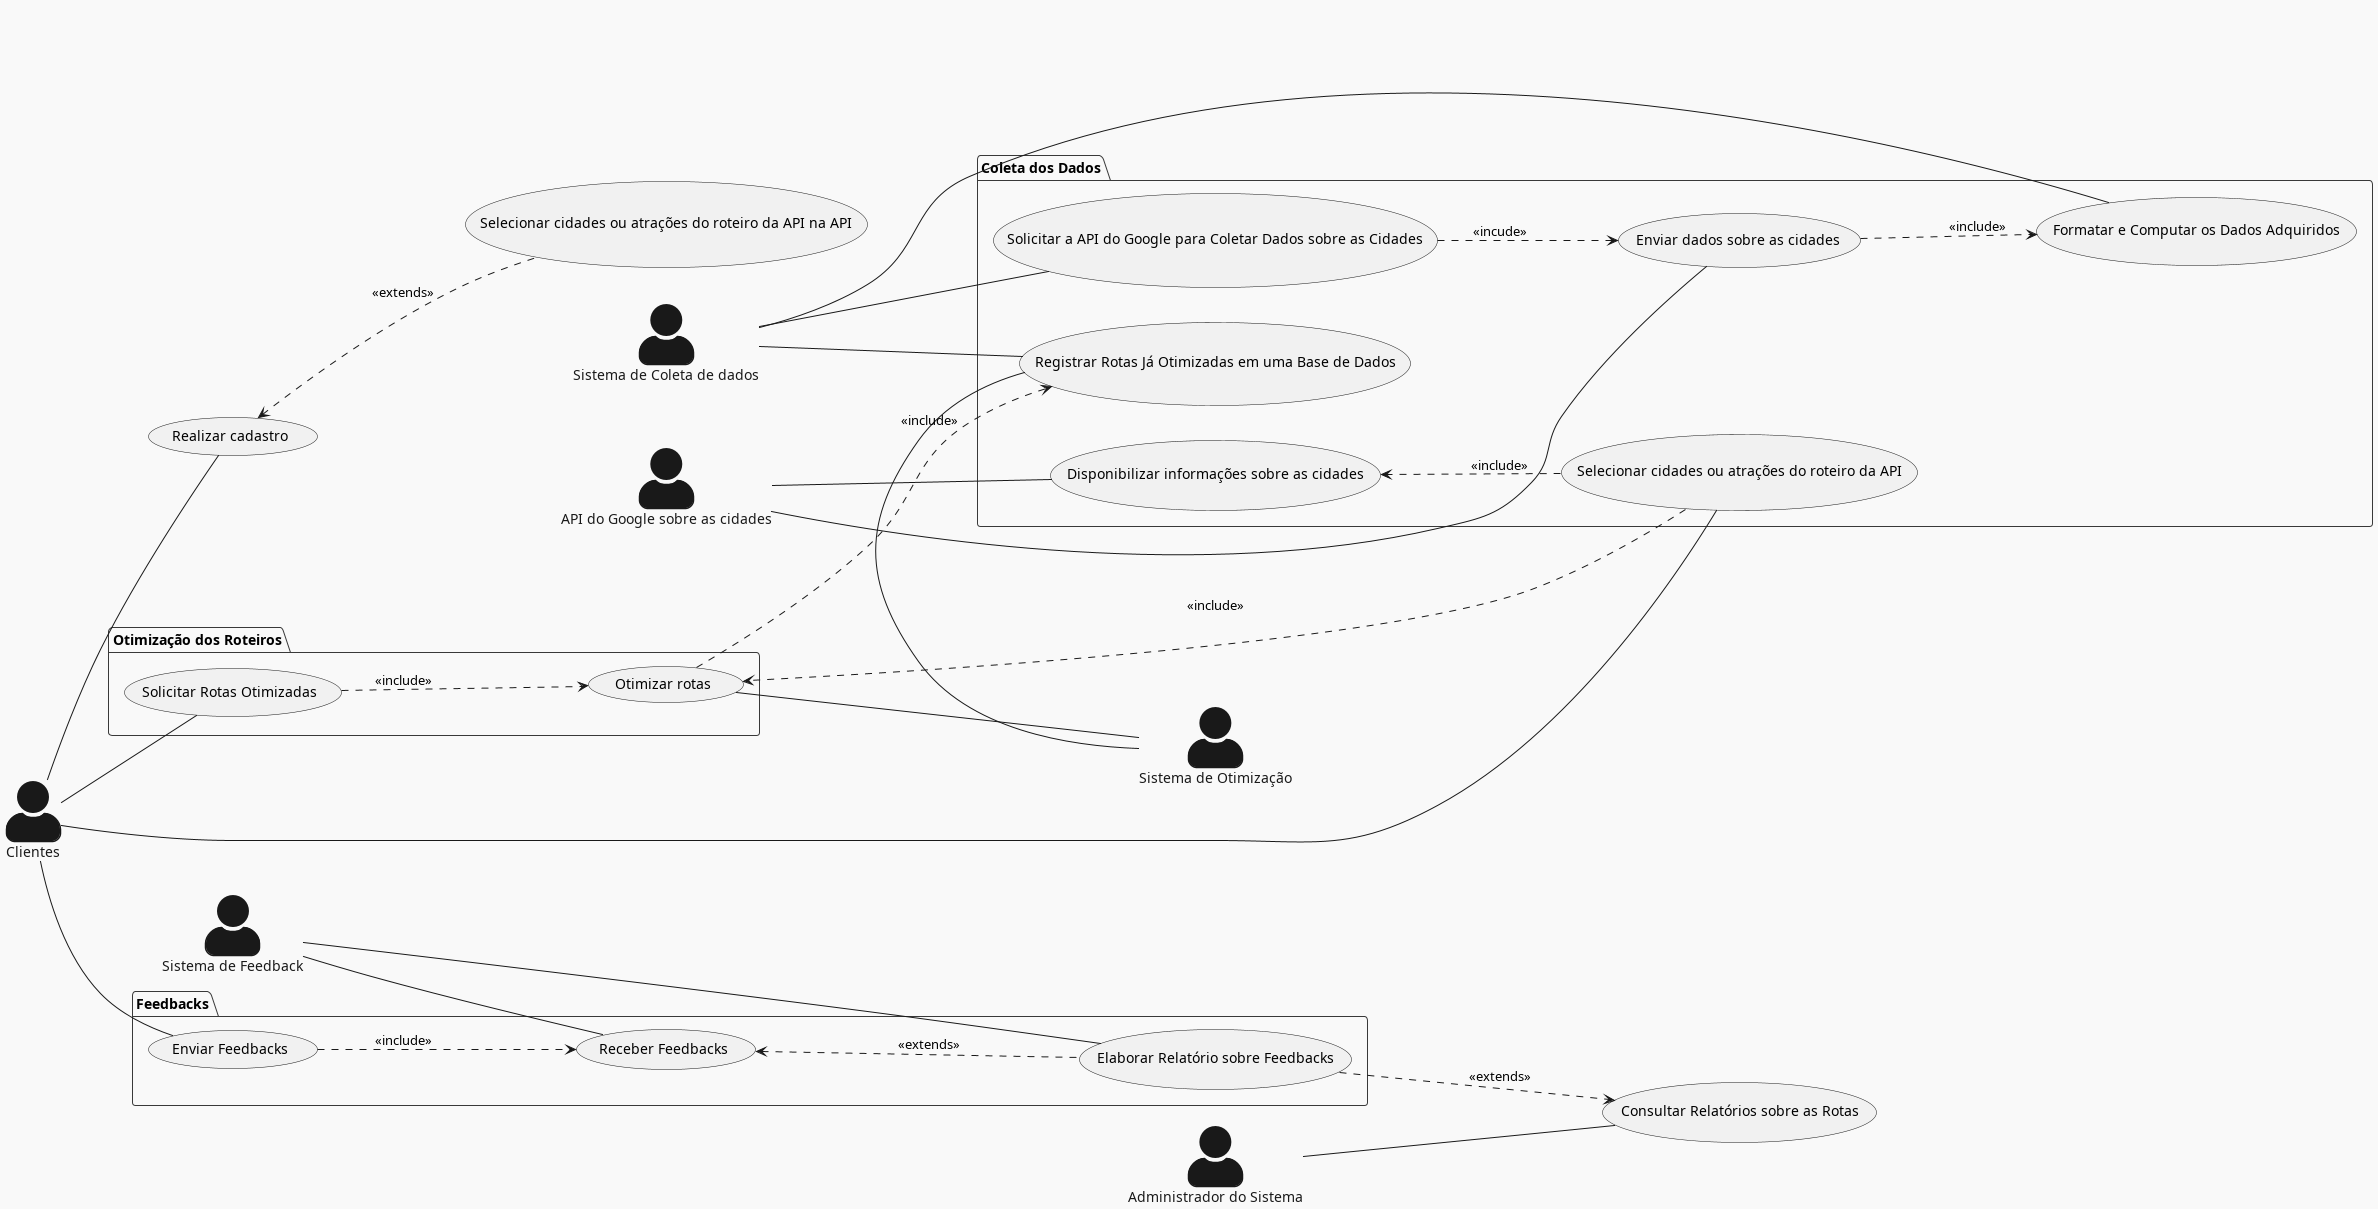
\includegraphics[scale=0.22]{Diagramas/DCU.png}\\
    \caption*{Fonte: Elaborado pelos autores}
\end{figure}

No diagrama de caso de uso, então, são observadas as interações entre os atores e as funcionalidades oferecidas pelo sistema de otimização de roteiros turísticos. O ator principal é denominado "Clientes", o qual interage com o sistema de diversas maneiras. Inicialmente, os clientes têm a capacidade de efetuar o cadastro no sistema, fornecendo suas informações pessoais para obter acesso às funcionalidades oferecidas.

Outra interação relevante é a capacidade dos clientes de "Enviar Feedbacks". Essa funcionalidade possibilita que os clientes forneçam suas opiniões, sugestões e avaliações sobre os roteiros turísticos e a experiência geral com o sistema. Esses feedbacks são valiosos para a melhoria contínua do sistema e para atender melhor às necessidades dos clientes.

Além do ator "Clientes", o "Administrador do Sistema" também desempenha um papel no diagrama. Ele tem acesso à funcionalidade de "Consultar Relatórios sobre as Rotas", que permite ao administrador visualizar relatórios detalhados elaborados sobre as rotas turísticas otimizadas. Tais relatórios são essenciais para o monitoramento do desempenho do sistema, a identificação de tendências e a tomada de decisões estratégicas.

O pacote "Otimização dos Roteiros" é um elemento-chave no diagrama, no qual o "Sistema de Otimização" desempenha um papel central. Ele oferece a funcionalidade de "Otimizar Rotas", a qual consiste no processo de otimização dos itinerários turísticos com base nas informações coletadas sobre as cidades ou atrações selecionadas. Essa funcionalidade é a essência do sistema.

O pacote "Coleta dos Dados" envolve o "Sistema de Coleta de Dados" e a "API do Google sobre as cidades". Esses atores trabalham em conjunto para coletar e disponibilizar informações detalhadas sobre as cidades e atrações turísticas. O sistema solicita dados relevantes à API do Google, a qual fornece as informações necessárias para que o sistema possa selecionar as cidades e atrações que atendam às preferências dos clientes.

Por fim, o pacote "Feedbacks" é responsável por coletar e armazenar os feedbacks enviados pelos clientes. O "Sistema de Feedback" possui a funcionalidade de "Armazenar dados do Feedback", permitindo que os feedbacks enviados pelos clientes sejam registrados para análise e futuras melhorias. Ademais, o sistema elabora relatórios sobre esses feedbacks, fornecendo informações importantes para avaliar a satisfação dos clientes e a eficácia do sistema em atender às suas expectativas.

Essas interações e funcionalidades detalhadas no diagrama de caso de uso oferecem uma visão clara das principais características do sistema de otimização de roteiros turísticos, enfatizando a personalização dos itinerários e a coleta de feedbacks como aspectos fundamentais para aprimorar a experiência dos clientes e garantir a eficiência do sistema

\subsection{Diagrama de Fluxo de Dados}

O diagrama de fluxo de dados é uma poderosa ferramenta de modelagem que descreve como as informações fluem dentro de um sistema, identificando as entradas, processamentos e saídas de dados. Nesta seção, apresentaremos o diagrama de fluxo de dados em três níveis (0, 1 e 2) do sistema de otimização de roteiros turísticos. O objetivo é fornecer uma visão detalhada das diferentes camadas do sistema, desde o nível mais abstrato até o mais detalhado.

\subsubsection{Nivel 0}

No DFD nível 0, foi representado a direção dos fluxos de informações que entram e saem do sitema principal, relacionando-os com os seus respectivos autores, os quais foram mostrados na Figura \ref{fig:DCU} 
\begin{figure}[H]
    \centering
    \caption{Diagrama Fluxo de Dados - Nível 0}
    \label{fig:DFD0}
    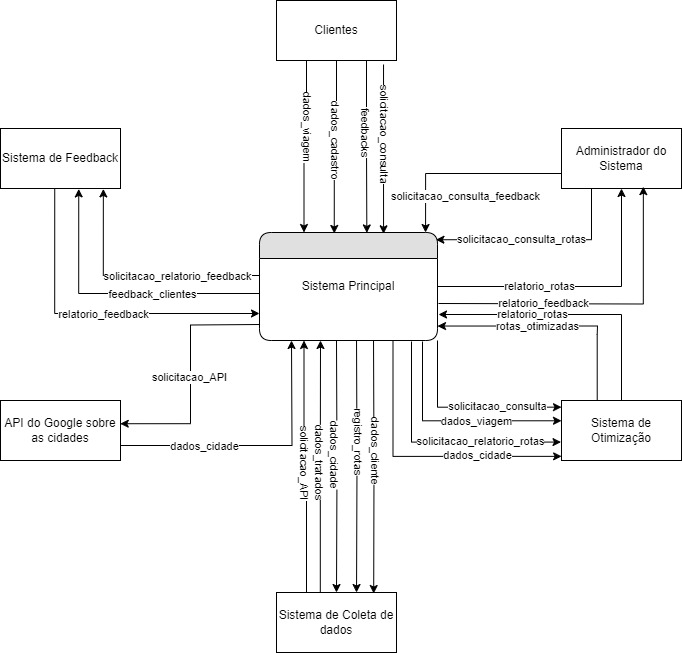
\includegraphics[scale=0.5]{Diagramas/DFD0.jpeg}\\
    \caption*{Fonte: Elaborado pelos autores, Figura completa disponível no apêndice}
\end{figure}

O sistema de otimização, por exemplo, envia para o sistema principal rotas otimizadas e recebe dados de cidades e solicitações de consulta. 


\subsubsection{Nivel 1}

Um Diagrama de Fluxo de Dados (DFD) de nível 1 é uma representação gráfica do sistema que descreve o fluxo de informações entre os principais processos e as principais entidades (ou atores) que interagem com o sistema.
No DFD de nível 1, o processo central do Diagrama de Contexto é decomposto em subprocessos menores, criando uma hierarquia de processos. Cada subprocesso representa uma parte específica do sistema e suas funcionalidades mais detalhadas. As setas representam os fluxos de dados entre os processos e as entidades, indicando a direção do fluxo das informações.

Esse nível de detalhamento torna o DFD de nível 1 mais compreensível e específico, permitindo que os analistas de sistemas e desenvolvedores tenham uma visão mais detalhada do funcionamento do sistema e das interações entre seus componentes.

Geralmente, em um DFD de nível 1, os processos principais são numerados, e as entradas e saídas de cada processo são identificadas por nome e direção do fluxo de dados. Isso ajuda a entender como as informações são processadas e compartilhadas entre os diferentes elementos do sistema.

\begin{figure}[H]
    \centering
    \caption{Diagrama Fluxo de Dados - Nível 1}
    \label{fig:DFD1}
    
\includegraphics[scale=0.5]{Diagramas/DFD1.png}\\
    \caption*{Fonte: Elaborado pelos autores, Figura completa disponível no apêndice}
\end{figure}

As relações são representadas da mesma maneira que no diagrama de nível 0. Aqui, porém, estão representadas também as bases de dados que são necssárias para que o sistema funcione e como os dados fluem entre elas e os processos. No caso, elas estão representadas por duas linhas paralelas com o nome da base entre as linhas


\subsubsection{Nivel 2}

\begin{figure}[H]
    \centering
    \caption{Diagrama Fluxo de Dados - Nível 2}
    \label{fig:DFD2}
    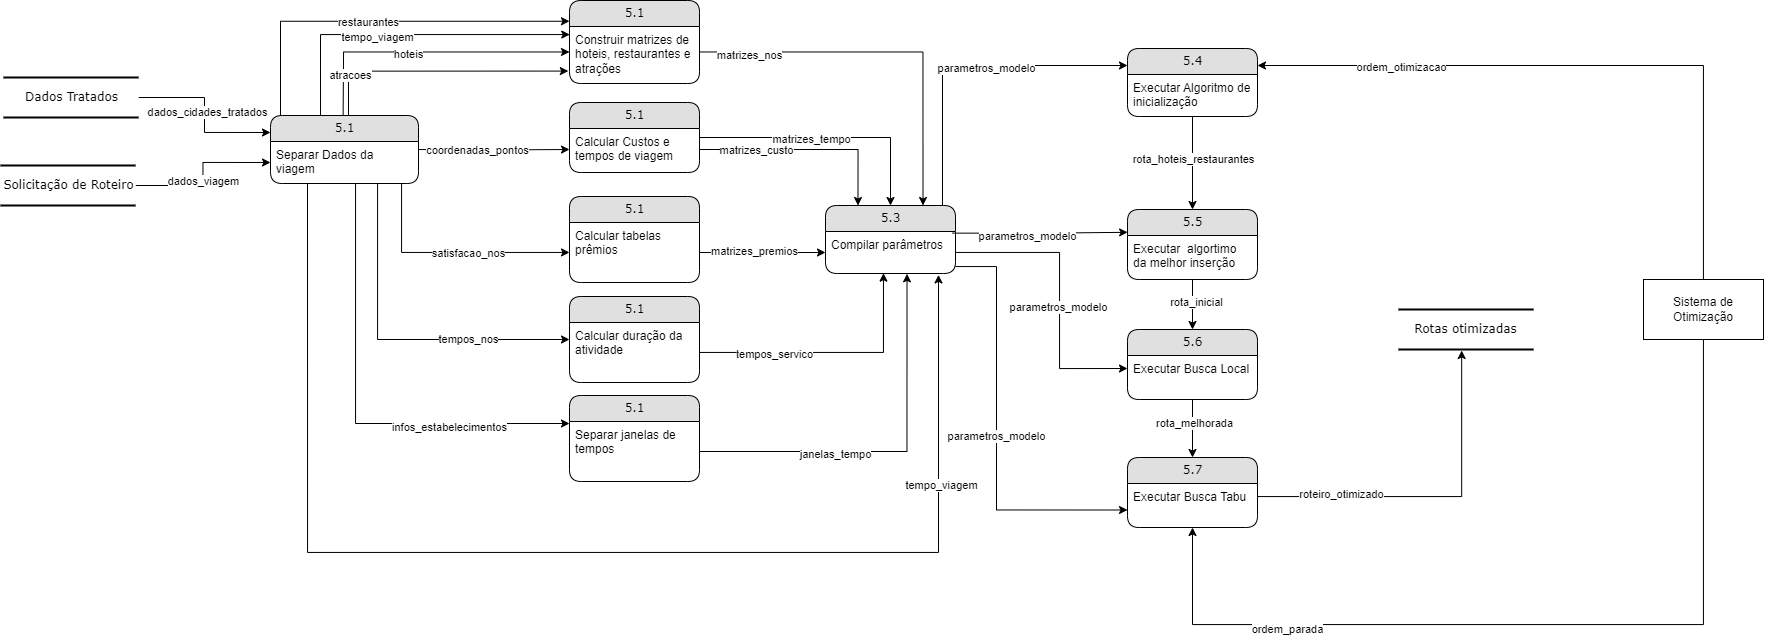
\includegraphics[scale=0.29]{Diagramas/DFD2.png}\\
    \caption*{Fonte: Elaborado pelos autores, Figura completa disponível no apêndice}
\end{figure}


\subsection{Diagrama de Entidade Relacionamento}

\begin{figure}[H]
    \centering
    \caption{Diagrama de Entidade Relacionamento}
    \label{fig:DER}
    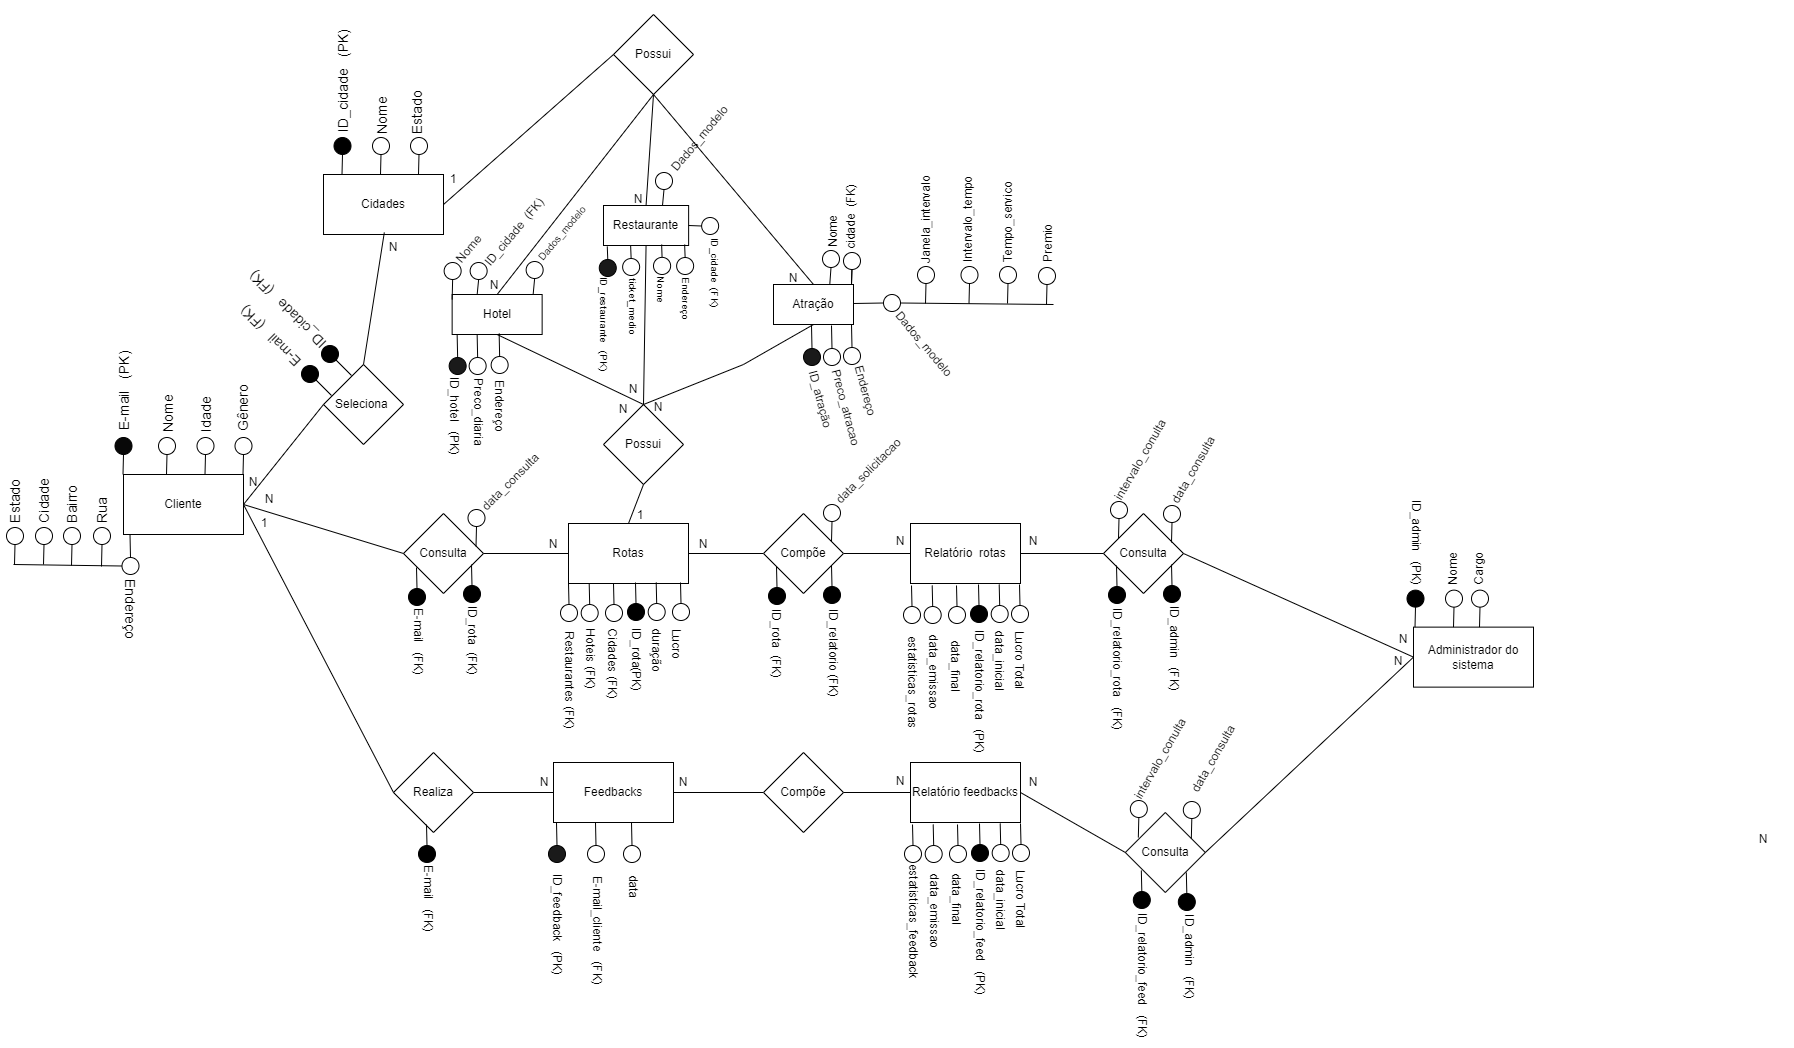
\includegraphics[scale=0.3]{Diagramas/DER.png}\\
    \caption*{Fonte: Elaborado pelos autores, Figura completa disponível no apêndice}
\end{figure}

O diagrama busca fornecer informações sobre como as entidades se relacionam dentro do sistema. A entidade "cliente" seleciona a entidade "Cidades" e essa seleção possui os atributos do email do cliente e do ID das cidades. Como um cliente pode selecionar várias cidades e uma cidade pode ser selecionaada por vários clientes, a relação construída é de "N para N". 

Outros aspectos que podem ser percebidos no diagrama é que rotas podem ser consultadas por clientes em alguma data e possuem Hoteis, atrações e Restaurantes. Estes, por sua vez, são "possuídos" (ou seja, pertencem) por uma cidade. Neste último caso, temos uma relação de "1 para N", porque uma cidade pode possuir várias dessas entidades, mas elas pertencem a uma, e somente uma, cidade. 

As demais relações podem ser entendidas e explicadas por vias análogas e a relação entre elas visualizada de maneira mais simples no modelo relacional. 



\subsection{Modelo Relacional}


\begin{figure}[H]
    \centering
    \caption{Modelo relacional}
    \label{fig:DER}
    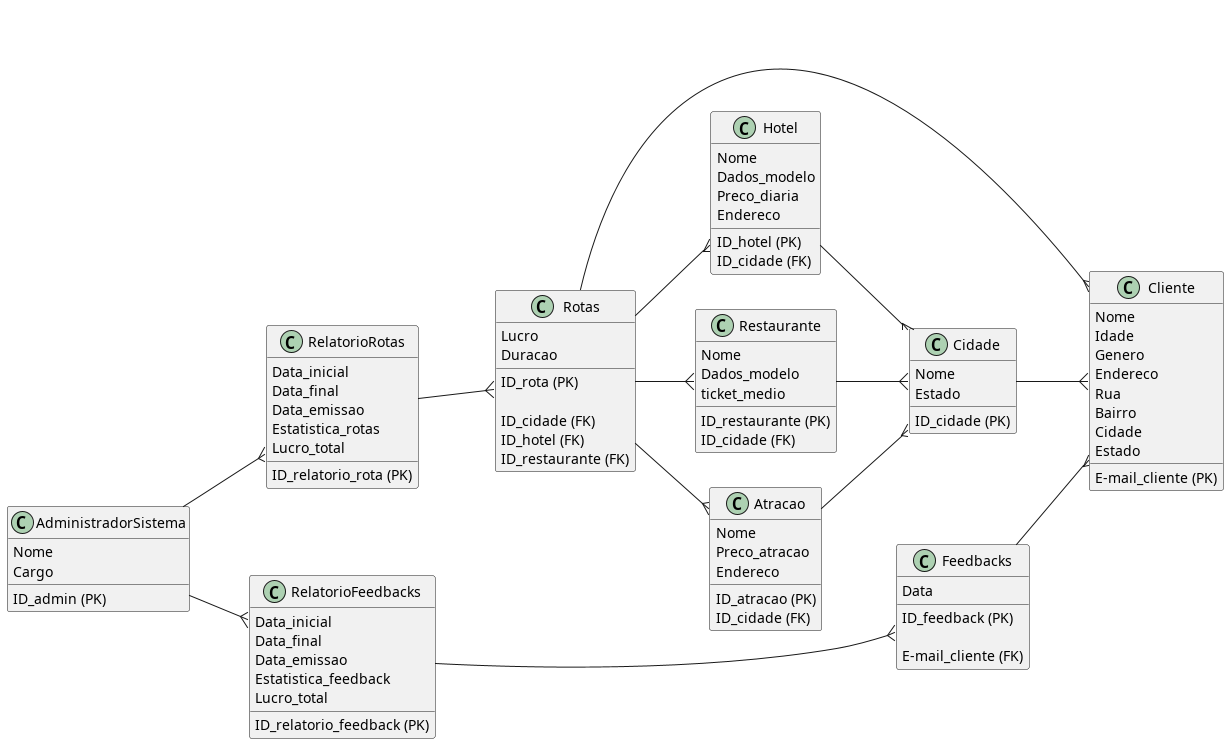
\includegraphics[scale=0.42]{Diagramas/Relacional.png}\\
    \caption*{Fonte: Elaborado pelos autores, Figura completa disponível no apêndice}
\end{figure}

O modelo relacional apresentado descreve a estrutura de dados do sistema de otimização de roteiros turísticos em PlantUML. Nesse modelo, temos diversas classes que representam as principais entidades do sistema, suas atribuições e relacionamentos entre si.

As classes principais incluem:
\begin{enumerate}
    \item \textbf{Cliente}: Representa os clientes do sistema e suas informações pessoais, como e-mail, nome, idade, gênero e endereço.
    \item \textbf{Cidade}: Refere-se às cidades cadastradas no sistema, com atributos como ID da cidade, nome e estado.
    \item \textbf{Hotel}: Descreve os hotéis disponíveis nas cidades do sistema, com informações como ID do hotel, nome, ID da cidade, dados do modelo, preço da diária e endereço.
    \item \textbf{Restaurante}: Representa os restaurantes presentes nas cidades, com atributos como ID do restaurante, nome, ID da cidade, dados do modelo e ticket médio.
    \item \textbf{Atração}: Refere-se às atrações turísticas nas cidades, com atributos como ID da atração, nome, ID da cidade, preço da atração e endereço.
    \item \textbf{Rotas}: Representa as rotas turísticas criadas pelo sistema, com informações como ID da rota, ID da cidade, ID do hotel, ID do restaurante, lucro e duração.
    \item \textbf{RelatorioRotas}: Descreve os relatórios gerados para as rotas, contendo ID do relatório, data inicial, data final, data de emissão, estatísticas das rotas e lucro total.
    \item \textbf{Feedbacks}: Representa os feedbacks enviados pelos clientes, com atributos como ID do feedback, e-mail do cliente e data do feedback.
    \item \textbf{RelatorioFeedbacks}: Descreve os relatórios gerados para os feedbacks, contendo ID do relatório, data inicial, data final, data de emissão, estatísticas dos feedbacks e lucro total.
    \item \textbf{AdministradorSistema}: Refere-se aos administradores do sistema, com informações como ID do administrador, nome e cargo.
\end{enumerate}

Os relacionamentos entre as classes são representados por associações. Por exemplo:
\begin{itemize}
    \item \textbf{Cliente} está associado à \textbf{Cidade}, \textbf{Rotas} e \textbf{Feedbacks}, indicando que um cliente pode estar relacionado a várias cidades, rotas e feedbacks.
    \item \textbf{Cidade} possui associações com \textbf{Hotel}, \textbf{Restaurante} e \textbf{Atração}, mostrando que uma cidade pode ter vários hotéis, restaurantes e atrações associados a ela.
    \item \textbf{Rotas} está associado a \textbf{Hotel}, \textbf{Atração} e \textbf{Restaurante}, indicando que uma rota pode incluir vários hotéis, atrações e restaurantes.
    \item \textbf{RelatorioRotas} está associado a \textbf{Rotas}, significando que um relatório de rotas pode abranger várias rotas.
    \item \textbf{RelatorioFeedbacks} está associado a \textbf{Feedbacks}, indicando que um relatório de feedbacks pode conter vários feedbacks.
    \item \textbf{AdministradorSistema} está associado a \textbf{RelatorioRotas} e \textbf{RelatorioFeedbacks}, mostrando que um administrador pode ter acesso a vários relatórios de rotas e feedbacks.
\end{itemize}

Esse modelo relacional descreve a estrutura de dados do sistema e os relacionamentos entre as entidades, fornecendo uma base sólida para a implementação do sistema de otimização de roteiros turísticos. Ele permite uma organização eficiente e precisa das informações, facilitando a consulta e manipulação dos dados, bem como a geração de relatórios para auxiliar a tomada de decisões.

